\subsection{Cantilever beam}
\paragraph{}
A two-dimensional cantilever beam subjected to a parabolic shear load at the free end is examined as shown
in fig.~\ref{qdt_fig:ex_cantilever_beam_geo_bc}.
    \begin{figure}[h!]
    \centering
        \scalebox{0.8}{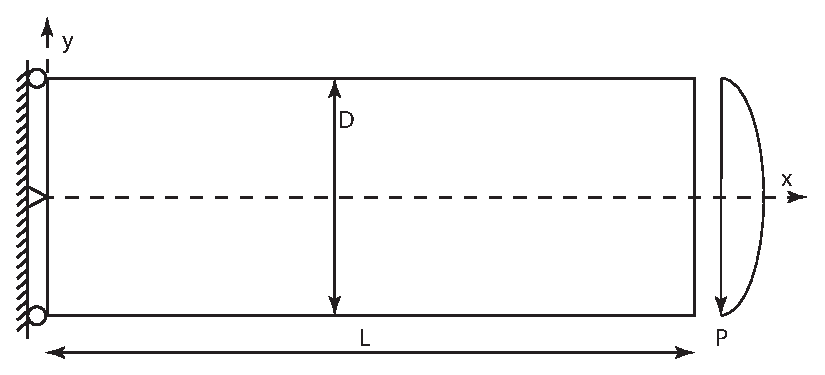
\includegraphics{isogeometric_sbfem/images/cantilever_beam_geo_bc.eps}}
        \caption{ Cantilever beam: Geometry and boundary conditions.}
        \label{qdt_fig:ex_cantilever_beam_geo_bc}
    \end{figure}

The geometry is: length $L=8m$, height $D=4m$.
The material properties are: Young’s modulus $E$ = $3 \times 10^7 N/m^2$ , Poisson’s ratio $ \nu =0.25$.
The parabolic shear force is $P = 250 N$.
The exact solutions for the displacements are given by \cite{Aug2008} as eq.~\ref{iso_eq:cantilever_beam_displacement_solution}.
where $I=D^3/12$ is the moment of inertia, $\mean{E}=E$, $\mean{\nu}=\nu$ and $\mean{E}=E/(1-\nu^2)$, $\mean{\nu}=nu/(1-nu)$ for plane stress and plane strain condition respectively.
The stress $\sigma$ can be expressed as \cite{Aug2008} as eq.~\ref{iso_eq:cantilever_beam_stress_solution}.
The strain energy can be derived from eq.~\ref{iso_eq:cantilever_beam_stress_solution} and eq.~\ref{iso_eq:cantilever_beam_displacement_solution} as eq.~\ref{iso_eq:cantilever_beam_energy_solution}.

\paragraph{}
In this example, rigid body motion is constrained by fixing 3 DOF on the left edge of the beam.
$u_x=0$ for points at $(0,-D/2)$ and $(0,D/2)$ and $u_y =0$ for point at $(0,0)$.
Stress from analytical solution in eq.~\ref{iso_eq:cantilever_beam_stress_solution} are applied on the boundary.

\paragraph{}
Due to the fact that the geometry of the cantilever beam can be described by four points and four straight lines, drawing in AutoCAD may not be necessary.
As a result, the input geometry is defined manually.
Generated background mesh, coloring and the final result with $res=32$, $s_{max}=16$ and $s_{min}=1$ are shown in fig.~\ref{qdt_fig:ex_cantilever_beam_background_mesh}, fig.~\ref{qdt_fig:ex_cantilever_beam_mesh_coloring} and fig.~\ref{qdt_fig:ex_cantilever_beam_mesh_final}.

    \begin{figure}
        \centering
        \scalebox{0.6}{
            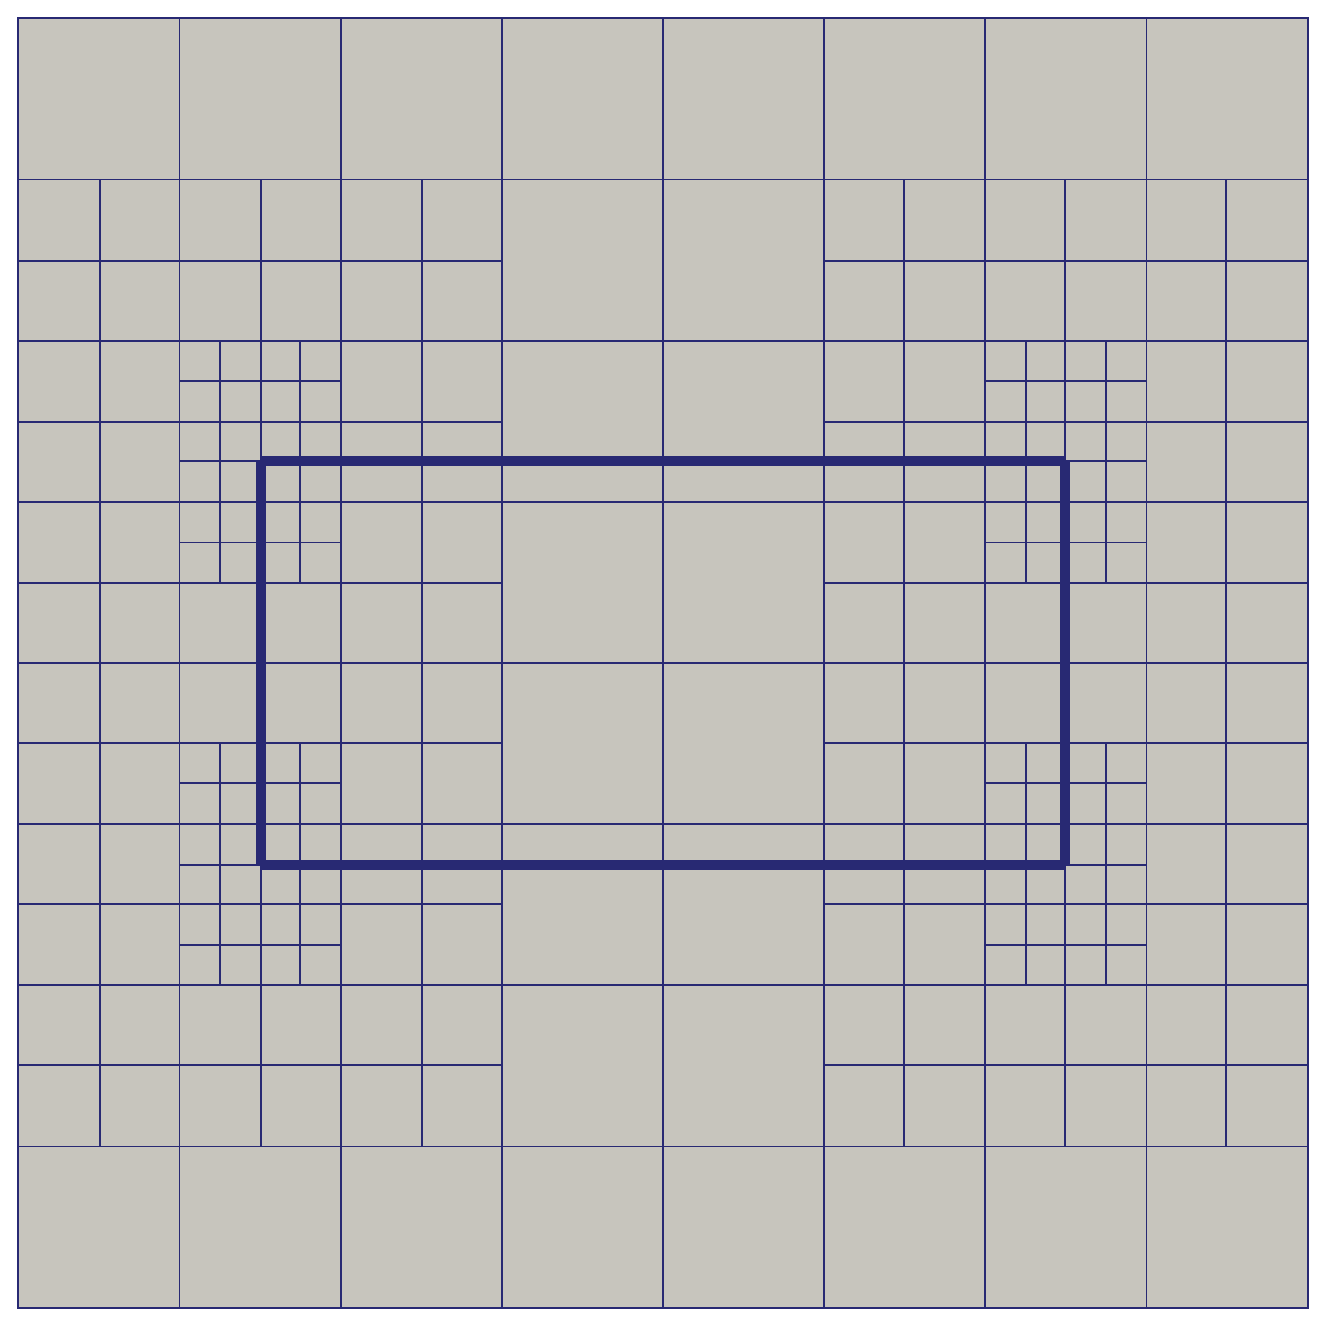
\includegraphics{quadtree/ex_images/cantilever_background_mesh.eps}
        }
        \caption[Background mesh of cantilever beam]{Background mesh of cantilever beam : Bold lines represents the input geometry}
        \label{qdt_fig:ex_cantilever_beam_background_mesh}
    \end{figure}

    \begin{figure}
        \centering
        \scalebox{0.6}{
            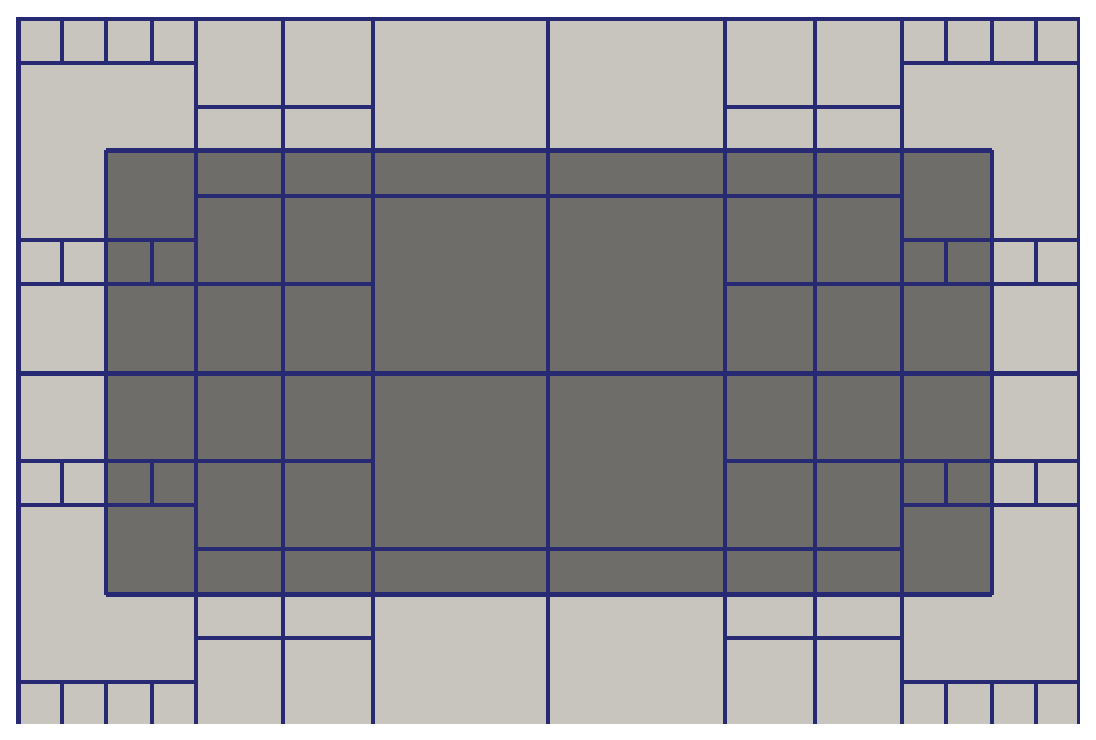
\includegraphics{quadtree/ex_images/cantilever_coloring.eps}
        }
        \caption[Mesh coloring of cantilever beam]{Mesh coloring of cantilever beam : Grey area represents the cantilever beam}
        \label{qdt_fig:ex_cantilever_beam_mesh_coloring}
    \end{figure}

    \begin{figure}
        \centering
        \scalebox{0.5}{
            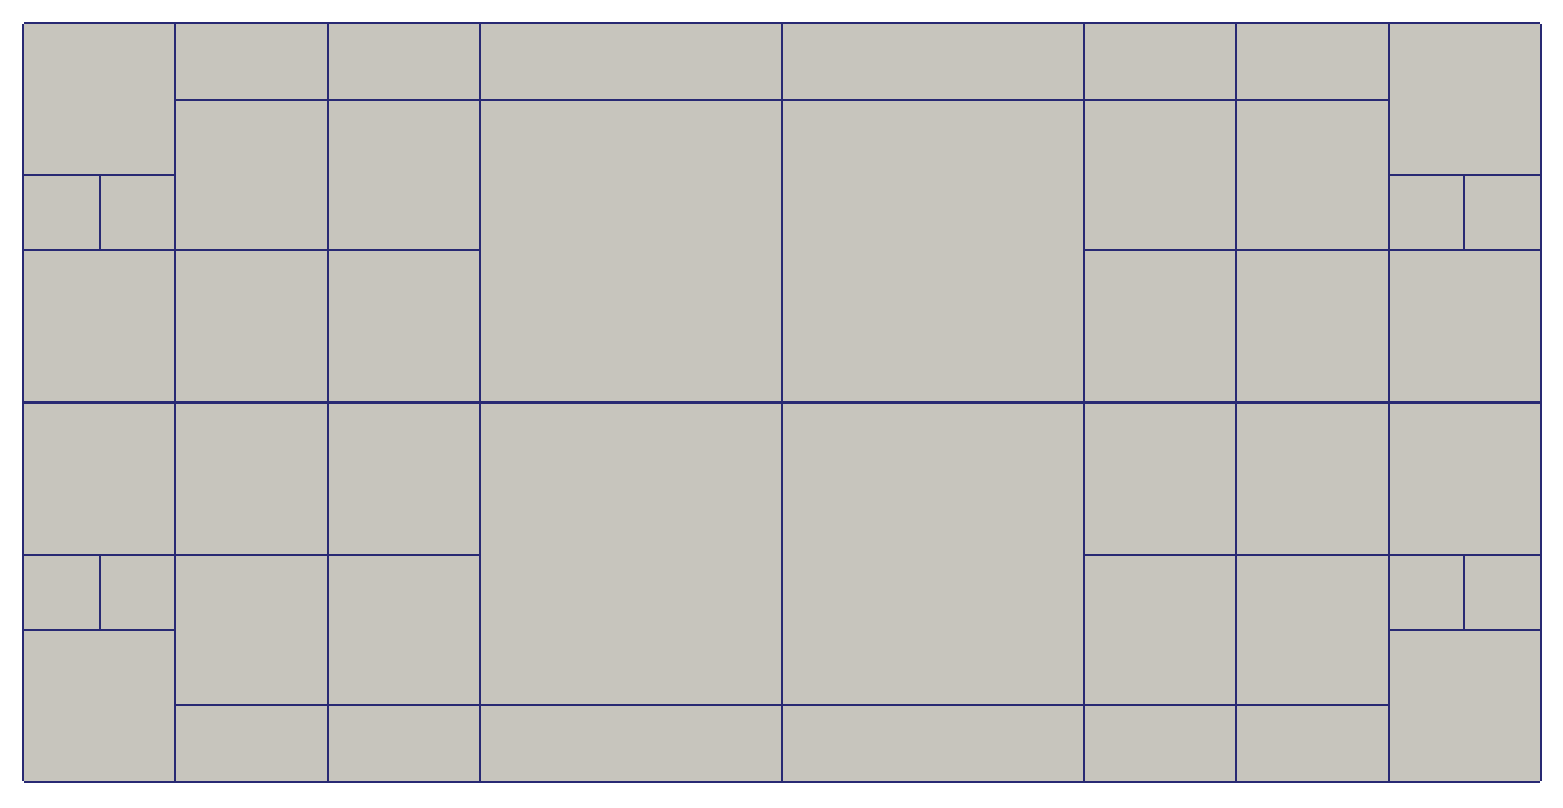
\includegraphics{quadtree/ex_images/cantilever_final_mesh.eps}
        }
        \caption[Final mesh of cantilever beam]{Final mesh of cantilever beam}
        \label{qdt_fig:ex_cantilever_beam_mesh_final}
    \end{figure}
% DOF err
% 146 - 0.019587 (32,16)
% 178 - 0.0082845 (32,2)
% 438 - 0.0027044 (64,2)
% 1658- 0.00066929 (128,2)
\paragraph{}
Mesh with different parameters are plotted in fig.~\ref{qdt_fig:ex_cantilever_mesh_all} and the convergence study is plotted in fig.~\ref{qdt_fig:ex_cantilever_mesh_conv}

    \begin{figure}[!ht]
        \begin{subfigure}[b]{1\linewidth}
            \centering
            \scalebox{0.4}{
                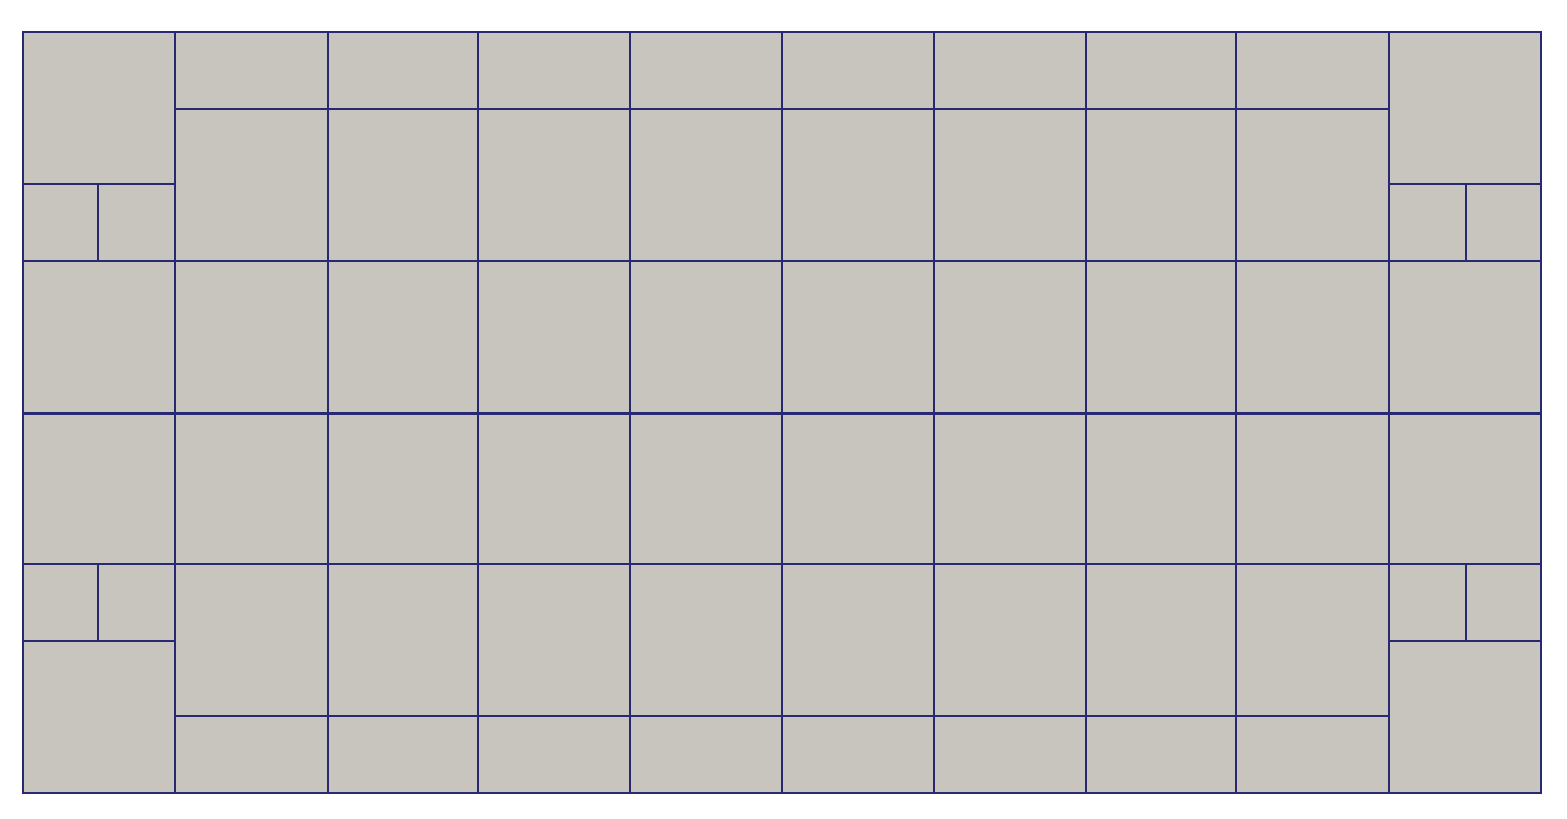
\includegraphics{quadtree/ex_images/qdt_cantilever_mesh_178.eps}
            }
            \caption{Mesh with $res=32$, $s_{max}=2$, 178 DOFs}
        \end{subfigure}
        \\
        \begin{subfigure}[b]{1\linewidth}
            \centering
            \scalebox{0.4}{
                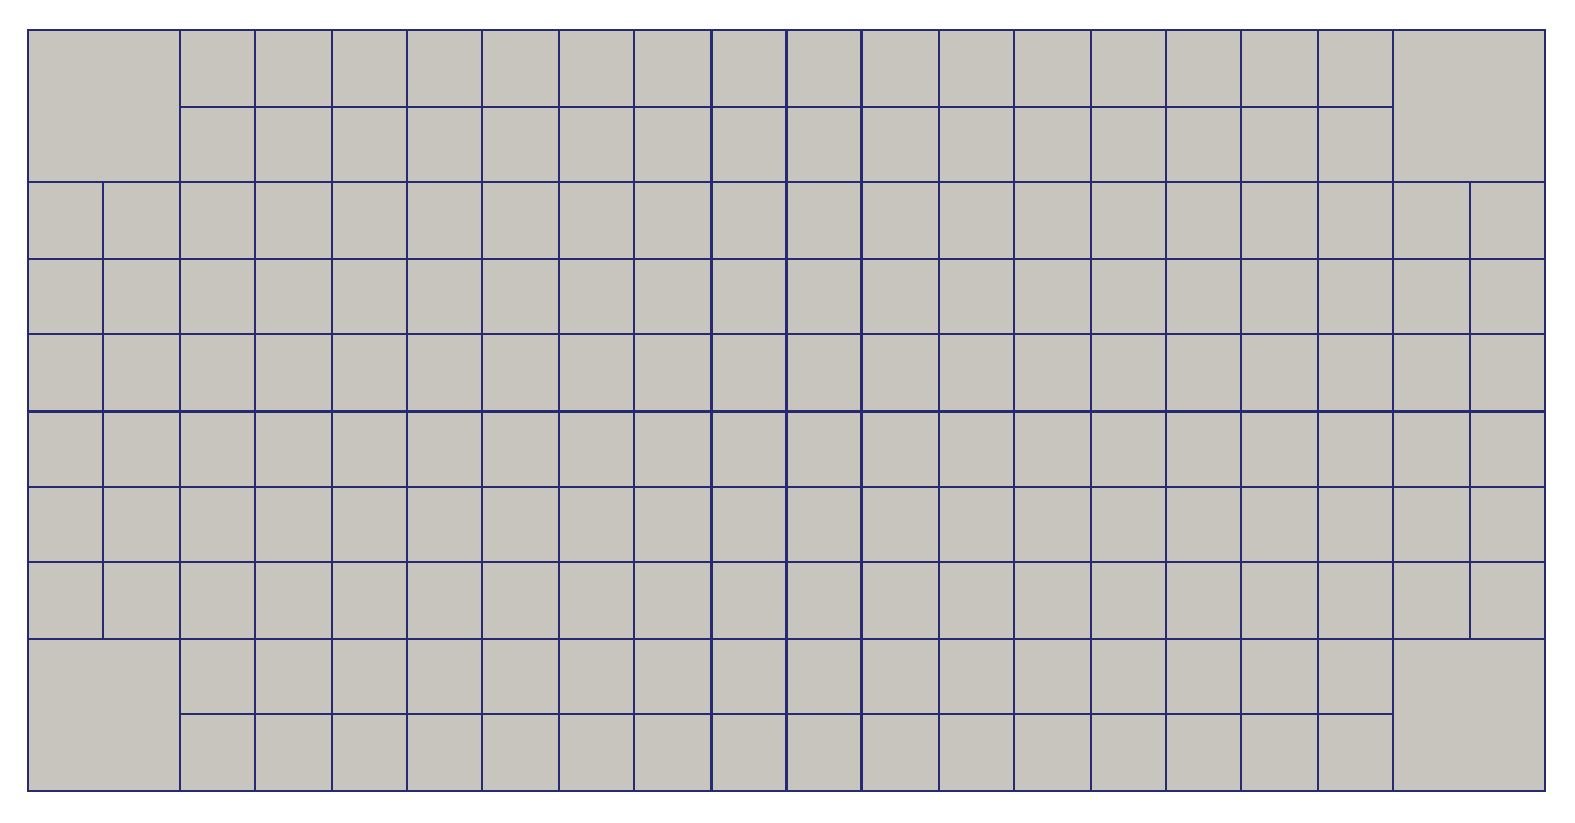
\includegraphics{quadtree/ex_images/qdt_cantilever_mesh_438.eps}
            }
            \caption{Mesh with $res=64$, $s_{max}=2$, 438 DOFs}
        \end{subfigure}
        \\
        \begin{subfigure}[b]{1\linewidth}
            \centering
            \scalebox{0.4}{
                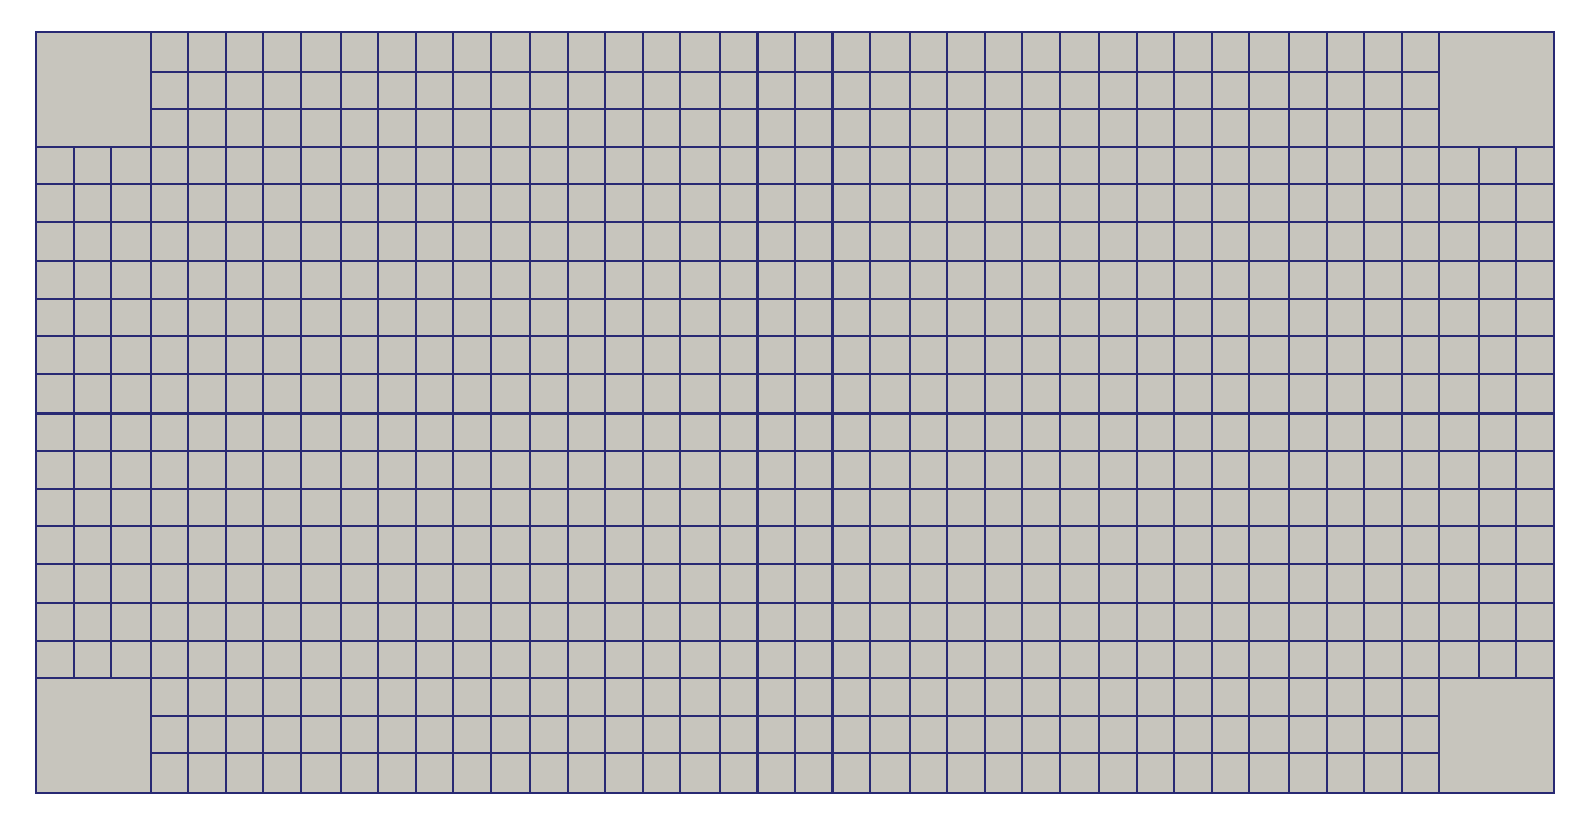
\includegraphics{quadtree/ex_images/qdt_cantilever_mesh_1658.eps}
            }
            \caption{Mesh with $res=128$, $s_{max}=2$, 1658 DOFs}
        \end{subfigure}
        \caption[Mesh of the cantilever beam]{Mesh of the cantilever beam}
        \label{qdt_fig:ex_cantilever_mesh_all}
    \end{figure}


    \begin{figure}[H]
        \centering
        \scalebox{0.75}{
            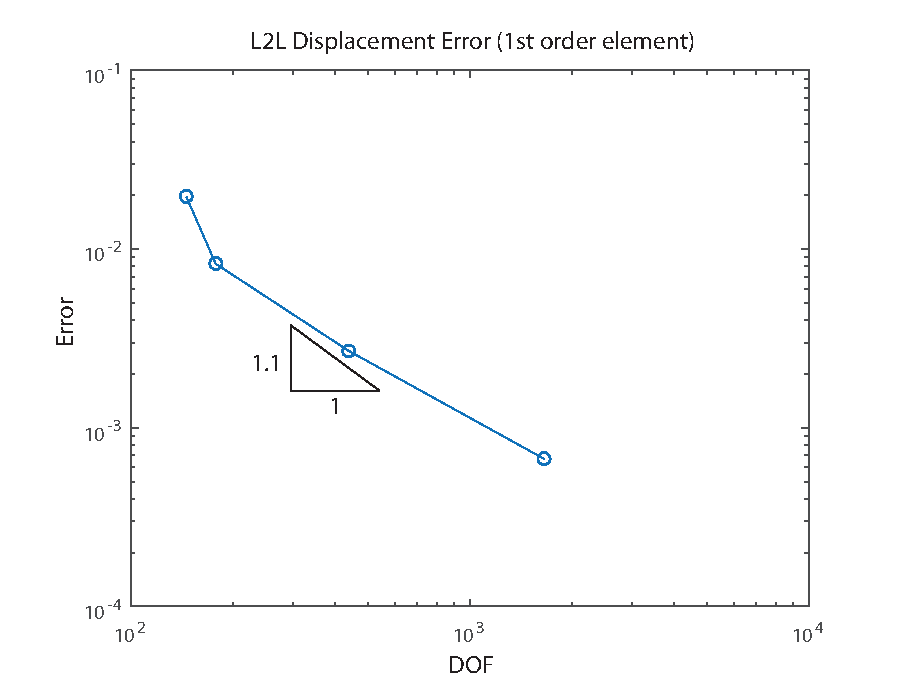
\includegraphics{quadtree/ex_images/qdt_cantilever_conv.eps}
        }
        \caption[Convergence of the cantilever beam]{Convergence of the cantilever beam}
        \label{qdt_fig:ex_cantilever_mesh_conv}
    \end{figure}

    
\pagebreak